\section{舞踊分類ネットワーク}

\subsection{モデル概要}
入力された動画を[優美なダンス,普通のダンス,その他の動作]に分類するために,
\begin{enumerate}
  \item 動画を下記で説明する二値化手法で編集する.
  \item 二値データと,それに対応するピクセル番号を畳み込む.
  \item 二つのデータを足し合わせる.
  \item Transformer Encoderに通した後,全結合し,Softmaxにかける.
\end{enumerate}
のようにネットワーク内で計算した.
最適化アルゴリズムにAdam\cite{adam},損失関数に交差エントロピー誤差(\ref{entropy})を使用した.
\begin{equation}
  H(p, q) = -\sum_{i}p_i\log q_i
  \label{entropy}
\end{equation}

\subsection{使用する動画データ}
\begin{table}[b]
  \begin{center}
    \begin{tabular}{|c|c|c|} \hline
      \ & 学習用 & 推論用 \\ \hline
      優美なダンス
        & \cite{jpn}\cite{china}\cite{ballet}\cite{thai}\cite{jpn2}
        & \cite{balletgroup}\cite{jpngroup}\cite{chinagroup}\cite{belly}
      \\ \hline
      普通のダンス
        & \cite{ariana}\cite{kadokawa}\cite{bts}\cite{manolo}\cite{aito}
        & \cite{btsgroup}\cite{arashi}\cite{hyoga}\cite{legit}
      \\ \hline
      その他の動作
        & \cite{radio}\cite{posing}\cite{boxing}\cite{running}\cite{shinkokyu}\cite{leaves}
        & \cite{radio2}
      \\ \hline
    \end{tabular}
  \end{center}
  \caption{使用した動画データ}
  \label{video_data}
\end{table}

動画は表\ref{video_data}を使用した.優美な動画の選定方法は,youtubeで優美,美しいなどの
キーワードで検索し,再生回数の多く,視聴した時に優美であると感じたものを使用した.
一つの国,舞踊の種類では目的である網羅的な学習を達成できないため,古今東西の舞踊を使用した.
普通のダンスでは同じようにダンスなどのキーワードを持ち,再生回数が多く,
視聴した時にダンスであると感じたものを使用した.その他の動作はランニングや体操など,
日常的な動作を使用した.再生回数が多いものを使用する理由は,その舞踊のエキスパートの動作を
できるだけ使用したかったからである.再生回数が多いということは,それだけ不特定多数から
注目を浴びている,感動を与えていると考えられ,その動作の熟練者である可能性が高いと考えた.

動画の編集方法は,まず,動画サイズを均一にするために,縦横64ピクセルに縮小した.
縦横短い方を基準に長い方の両端を切り出し,OpenCVのresize\cite{resize}にかけた.
畳み込みでは正方形のフィルタを用いるため,動画サイズを正方形にする必要があった.
リサイズ後の動画を確認した結果,64ピクセルが動作が確認できる最も小さなサイズであった.

次に,動画を二値化した.グレースケールに次元を落とした動画の1フレームごとの画像全体の平均をとった.
その平均より値の低いピクセルを255,高いピクセルを0にした.人体や服の色は
背景色より暗いことが多かったのでここではソフトに二値化した.

最後に図\ref{choice}のように白画素の制限を行なった.
先ほど二値化した動画の1ピクセルのフレーム長の配列を取り出した.
その配列の平均を取り,255/4に近い順で,そのフレームでの対象が黒画素であった場合はカウントせず,
500画素まで採用した.閾値255/4はいくつか動画に制限処理を行なった中で最も汎用的に
人体の輪郭を得ることができたためこのような値を用いた.

\begin{figure}[b]
  \begin{center}
    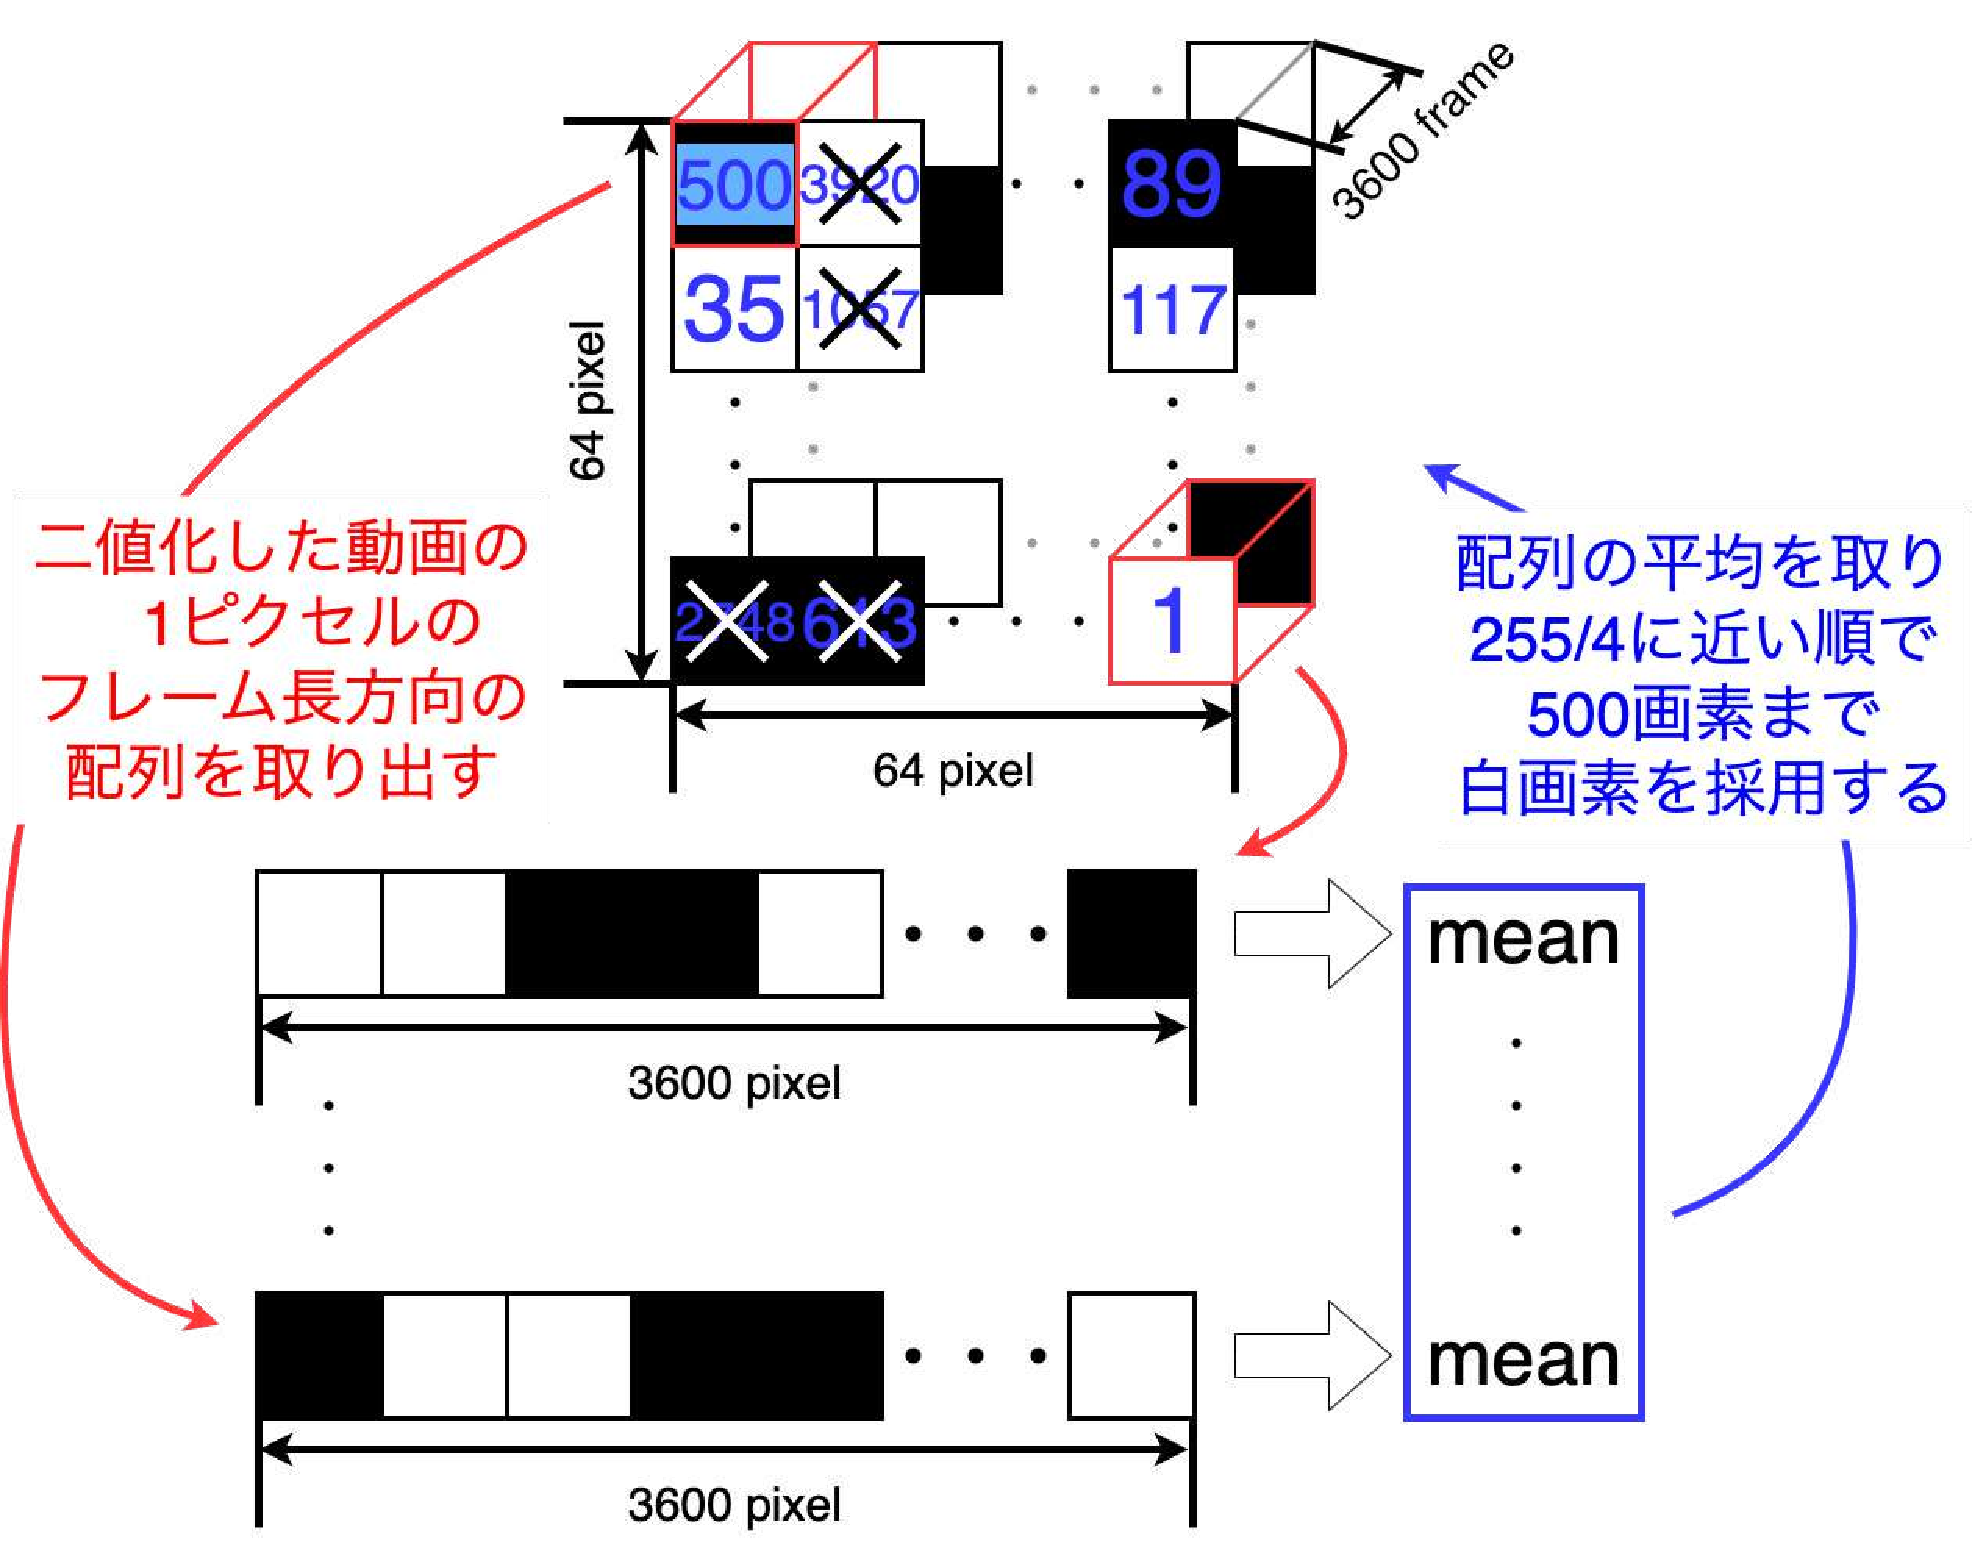
\includegraphics[width=100mm]{images/chart/choice.pdf}
  \end{center}
  \caption{白画素の制限方法}
  \label{choice}
\end{figure}

\clearpage

\subsection{ネットワーク構造}

\subsection{精度}